\documentclass[14pt]{extreport}

\usepackage{fancyhdr}
\pagestyle{fancy}
\fancyhf{}
\renewcommand{\headrulewidth}{0pt}
\cfoot{\thepage}

\usepackage[table]{xcolor}
\usepackage{new_gost}
\usepackage{graphicx}
\usepackage[toc, page]{appendix}
\usepackage{multicol}

\begin{document}
\setlength{\parindent}{1.25cm} % для шрифта 14pt
\pagestyle{empty}

\includepdf[pages=-,pagecommand={}]{TitulBD_2.pdf}

\pagestyle{plain} % включаем нумерацию

\tableofcontents

\intro\label{intro}
%\chapter{ВВЕДЕНИЕ}

Ведение складского учета бытовой техники - это необходимое условие для эффективного управления складскими запасами. Ведение учета позволяет получить точную информацию о количестве и типе техники на складе, а также контролировать ее движение и избежать потерь или краж.

Кроме того, ведение складского учета позволяет оптимизировать процесс продаж и сбыта, учитывая сезонность спроса на различные виды техники и особенности рынка. Например, знание того, какие товары на складе наиболее популярны в конкретный период, позволяет оперативно реагировать на изменения спроса и увеличивать прибыльность бизнеса.

Более того, точный учет бытовой техники на складе помогает улучшить качество обслуживания клиентов. Знание наличия техники на складе позволяет оперативно реагировать на запросы и желания клиентов, улучшать время доставки и решать проблемы с запасами.

В целом, ведение складского учета бытовой техники - это необходимый элемент эффективного управления складскими запасами, что позволяет улучшить качество обслуживания клиентов, увеличить прибыльность бизнеса и оптимизировать процесс продаж и сбыта. Склады бытовой техники являются ключевой составляющей современной розничной торговли. Они обеспечивают постоянное наличие разнообразной бытовой техники, такой как холодильники, стиральные машины и другие устройства, гарантируя доступность продукции для потребителей в любое время. Это позволяет управлять запасами, удовлетворять спрос и обеспечивать клиентов нужными товарами, способствуя повышению эффективности бизнеса и удовлетворению потребностей покупателей.


\newpage
%\begin{justforlargetext}
%\large
%\textbf{ЦЕЛЬ И ЗАДАЧИ}\\
%\end{justforlargetext}
\chapter{ЦЕЛЬ И ЗАДАЧИ}
\textbf{Целью }данного исследования является практическое освоение этапов создания надежной базы данных для управления складом бытовой техники.


\textbf{Мы ставим перед собой следующие задачи: }


1. Создать и описать углублённый сценарий базы данных, отражающий информацию о каждом виде бытовой техники.


2. Выделить ключевые объекты системы, такие как конкретные модели бытовой техники, данные о поставщиках, хранении и продажах. 


3. Провести логическое проектирование, включающее нормализацию данных для достижения оптимальной формы вследствие анализа 1НФ, 2НФ и 3НФ, а также описание ключевых ограничений и возможную денормализацию для улучшения эффективности. 


4. Сформировать физическую модель базы данных, определяющую структуру таблиц, связи между ними и хранящую информацию о технике, поставках, клиентах и продажах. 


5. Разработать основные запросы к базе данных, которые позволят оперативно получать информацию о наличии техники, популярности определенных товаров в разные периоды времени и другую важную аналитику (информация о сотруднике, накладная и т.д.) 


Исходя из значимости точного складского учета для бытовой техники, данная работа направлена на улучшение качества обслуживания клиентов, оптимизацию процесса продаж и сбыта, а также на повышение эффективности управления запасами и предотвращение потерь или несанкционированных перемещений товаров.


\newpage
%\begin{justforlargetext}
%\large
%\textbf{ВЫПОЛНЕНИЕ}\\
%\end{justforlargetext}
\chapter{ВЫПОЛНЕНИЕ}

%\begin{justforlargetext}
%\large
%\textbf{Создание углубленного сценария базы данных}\\
%\end{justforlargetext}

\section{Создание углубленного сценария базы данных}

Объектом проекта является магазин бытовой техники, имеющий физические точки продажи. Когда речь идет о складской технике, учет на точечных магазинах является более актуальным, чем на онлайн-магазинах по нескольким причинам:

1. Физические склады: Точечные магазины имеют физические склады, где хранятся товары. В то время как в онлайн-магазинах товары хранятся на центральном складе и доставляются клиентам по мере необходимости. Поэтому учет складской техники на точечных магазинах является более актуальным.

2. Различные типы складской техники: Различные типы складской техники используются для различных целей, например, погрузочные машины используются для перемещения тяжелых грузов, а погрузчики с низким подъемом используются для перемещения грузов на низких высотах. На точечных магазинах обычно используется широкий спектр складской техники, поэтому учет их использования является более актуальным.

3. Контроль за состоянием техники: Точечные магазины обычно имеют своих сотрудников, которые могут следить за состоянием складской техники и проводить регулярное техническое обслуживание. В то время как в онлайн-магазинах такой контроль является более сложным, так как техника находится на центральном складе.

У магазина главной категорией покупателей являются индивидуальные покупатели.
Когда клиент делает заказ в базе данных регистрируются данные о покупателе, описание бытовой техники, информация о складе и т. д. Всё это фиксируется в накладной, где уже непосредственно сотрудник склада будет обрабатывать информацию. Так же для внутреннего учёта всегда есть полная информация о самом складе, о том, кто обрабатывает запрос

В целом, учет складской техники на точечных магазинах является более актуальным, так как они имеют физические склады и используют различные типы складской техники для различных целей.



\newpage
%\begin{justforlargetext}
%\large
%\textbf{Определение ключевых объектов системы}\\
%\end{justforlargetext}
\section{Интервью}

\textbf{Интервьюер:}

-Какие данные вы часто импортируете или экспортируете из системы?

\textbf{Менеджер:}

-Данные о клиентах, товарах, заказах, поставках и складских запасах могут быть импортированы и экспортированы. Это включает в себя информацию о наличии товаров на складе, данные о поставщиках, информацию о заказах и отгрузках. 


\textbf{Интервьюер:}

-С какими проблемами вы сталкиваетесь при работе с текущей базой данных?


\textbf{Менеджер:}

-На логической схеме видно множество связей между таблицами, что может привести к сложности управления целостностью данных. Кроме того, если база данных не оптимизирована для работы с большими объемами данных или высокой нагрузкой, могут возникнуть проблемы с производительностью, да и гарантия надежности сервера не подтверждена.


\textbf{Интервьюер:}

-Какие основные этапы процесса продажи в вашей компании?

\textbf{Менеджер:}

-Этапы включают управление клиентской информацией, учет товаров и категорий товаров, обработку заказов, логистику поставок и отгрузок. Весь процесс поддерживается данными, хранящимися и обрабатываемыми в различных связанных таблицах.


\textbf{Интервьюер:}

-Какие роли и уровни доступа вы видите для сотрудников в системе базы
данных?


\textbf{Менеджер:}

-Сотрудники склада, менеджеры по продажам и сотрудники отдела закупок имеют различные уровни доступа. Например, сотрудники склада имеют доступ к информации о товарах на складе, в то время как менеджеры по продажам работают с информацией о клиентах и заказах.


\textbf{Интервьюер:}

-Какие данные о клиентах вам важны для эффективной работы? Какие
данные обязательны для внесения в систему?


\textbf{Менеджер:}

-Важными данными о клиентах являются ФИО, контактный телефон и email. Обязательные данные для внесения в систему могут включать уникальный идентификатор клиента и контактную информацию для возможности связи и управления заказами.


\textbf{Интервьюер:}

-Опишите процесс, в котором вы обычно добавляете или изменяете данные в системе.


\textbf{Менеджер:}

-Процесс может включать внесение данных в таблицу клиентов или товаров через форму ввода, связывание заказов с клиентами и товаром, а также обновление данных о наличии товара на складе после отгрузки.


\textbf{Интервьюер:}

-Есть ли типы данных, которые требуют особой обработки, например, конфиденциальные или личные данные?


\textbf{Менеджер:}

-Конфиденциальные данные, такие как контактная информация клиентов и финансовые данные, должны обрабатываться с учетом политик безопасности. Это может включать ограничение доступа к данным, их шифрование и регулярное обновление политик безопасности.

%\section{Определение ключевых объектов системы}

% \textbf{Определение сущностей}

%В процессе разработки БД было выделено множество сущностей (рисунок 2). Были составлены таблицы для их описания.

\section{Определение категории типа данных для всех атрибутов каждой сущности}

\textbf{Используемые типы данных:}


- int – числовой


- text – символьный


- float – приближенный числовой


- date – дата

\vspace{1em}
\noindent
Таблица 1 - Товар
\begin{center}
\begin{longtable}{ |m{3.3cm}|m{3cm}|m{6cm}|m{1.8cm}| } 
 \hline
 Атрибуты & Тип & Описание & Обяз. \\ [0.5ex] 
 \hline\hline
 id & INT & Первичный ключ & \# \\
 \hline
 Наименование & TEXT & Наименование товара & * \\
 \hline
 Модель & TEXT & Название модели & * \\
 \hline
 Производитель & TEXT & Производитель товара & *\\ 
 \hline
 Количество\_
 
 на\_складе & INT & Количество единиц товара на складе & * \\
 \hline
 Категория\_id & INT & Номер категории товара (внешний ключ) & * \\ 
 \hline
 Поставщик\_id & INT & Номер поставщика товара (внешний ключ) & * \\ 
 \hline
 Накладная\_id & INT & Номер накладной товара (внешний ключ) & * \\ 
 \hline

 \hline
\end{longtable}
\end{center}

\newpage

\noindent
Таблица 2 - Клиент

\begin{center}
\begin{longtable}{ |m{3.3cm}|m{3cm}|m{6cm}|m{1.8cm}| } 
 \hline
 Атрибуты & Тип & Описание & Обяз. \\ [0.5ex] 
 \hline\hline
 id & INT & Первичный ключ & \# \\
 \hline
 Имя & TEXT & Имя клиента & * \\
 \hline
 Фамилия & TEXT & Фамилия клиента & * \\
 \hline
 Отчество & TEXT & Отчество клиента & 0 \\
 \hline
 Контактный\_
 
 телефон & TEXT & Номер телефона клиента & [\#] \\
 \hline
 Email & TEXT & Электронная почта клиента & * \\
 \hline
\end{longtable}
\end{center}
Один

\noindent
Таблица 3 - Накладная поставки
\begin{center}

\begin{longtable}{ |m{3.3cm}|m{3cm}|m{6cm}|m{1.8cm}| } 
 \hline
 Атрибуты & Тип & Описание & Обяз. \\ [0.5ex] 
 \hline\hline
 id & INT & Первичный ключ & \# \\
 \hline
 Дата & DATE & Дата поставки & * \\
 \hline
 Количество\_ 
 
 поставленного\_
 
 товара & INT & Количество единиц поставленного товара & * \\
 \hline
 Цена\_
 
 закупки & FLOAT & Цена закупки товаров  & * \\ 
 \hline
 Поставщик\_id & INT & Номер поставщика (внешний ключ) & * \\
 \hline
 Склад\_id & INT & Номер склада (внешний ключ) & * \\ 
 \hline
 Сотрудник\_
 
 id & INT & Номер сотрудника склада, подписавшего накладную(внешний ключ) & * \\ 
 \hline

 \hline
\end{longtable}
\end{center}


\newpage

\noindent
Таблица 4 - Отгрузка

\begin{center}
\begin{longtable}{ |m{3.3cm}|m{3cm}|m{6cm}|m{1.8cm}| } 
 \hline
 Атрибуты & Тип & Описание & Обяз. \\ [0.5ex] 
 \hline\hline
 id & INT & Первичный ключ & \# \\
 \hline
 Дата & DATE & Дата выполнения отгрузки & * \\
 \hline
 Количество\_
 
 проданного\_
 
 товара & INT & Количество проданных единиц товара & * \\
 \hline
 Цена\_
 
 продажи & FLOAT & Общая стоимость продажи товаров отгрузки & * \\
 \hline
 Клиент\_id & INT & Номер клиента (внешний ключ) & * \\
 \hline
 Товар\_id & INT & Номер товара (внешний ключ) & * \\
 \hline
 Склад\_id & INT & Номер склада (внешний ключ) & * \\
 \hline
 Сотрудник\_
 
 склада\_
 
 id & INT & Номер сотрудника, ответственного за отгрузку (внешний ключ) & * \\
 \hline
\end{longtable}
\end{center}



\noindent
Таблица 5 - Поставщик

\begin{center}
\begin{longtable}{ |m{3.3cm}|m{3cm}|m{6cm}|m{1.8cm}| } 
 \hline
 Атрибуты & Тип & Описание & Обяз. \\ [0.5ex] 
 \hline\hline
 id & INT & Первичный ключ & \# \\
 \hline
 Наименование & TEXT & Наименование компании поставщика & * \\
 \hline
 Контактная\_
 
 информация & TEXT & Контактная информация поставщика & * \\
 \hline
 Условия\_
 
 поставки & TEXT & Условия поставки товаров от поставщика & * \\
 \hline
\end{longtable}
\end{center}


\newpage

\noindent
Таблица 6 - Склад

\begin{center}
\begin{longtable}{ |m{3.3cm}|m{3cm}|m{6cm}|m{1.8cm}| } 
 \hline
 Атрибуты & Тип & Описание & Обяз. \\ [0.5ex] 
 \hline\hline
 id & INT & Первичный ключ & \# \\
 \hline
 Наименование & TEXT & Название склада & * \\
 \hline
 Улица & TEXT & Улица, на которой находится склад & * \\
 \hline
 Строение & TEXT & Строение, в котором находится склад & * \\
 \hline
 Вместимость & INT & Вместимость склада & * \\
 \hline
 Сотрудник\_
 
 id & INT & Номер сотрудника, работающего на складе (внешний ключ) & * \\
 \hline
\end{longtable}
\end{center}



\noindent
Таблица 7 - Сотрудник склада

\begin{center}
\begin{longtable}{ |m{3.3cm}|m{3cm}|m{6cm}|m{1.8cm}| } 
 \hline
 Атрибуты & Тип & Описание & Обяз. \\ [0.5ex] 
 \hline\hline
 id & INT & Первичный ключ & \# \\
 \hline
 Имя & TEXT & Имя клиента & * \\
 \hline
 Фамилия & TEXT & Фамилия клиента & * \\
 \hline
 Отчество & TEXT & Отчество клиента & 0 \\
 \hline
 Должность & TEXT & Должность сотрудника & * \\
 \hline
\end{longtable}
\end{center}

\newpage

\noindent
Таблица 8 - Категория товаров

\begin{center}
\begin{longtable}{ |m{3.3cm}|m{3cm}|m{6cm}|m{1.8cm}| } 
 \hline
 Атрибуты & Тип & Описание & Обяз. \\ [0.5ex] 
 \hline\hline
 id & INT & Первичный ключ & \# \\
 \hline
 Наименование & TEXT & Наименование категории & * \\
 \hline
 Описание & TEXT & Описание категории & * \\
 \hline
\end{longtable}
\end{center}


\noindent
Таблица 9 - Товар на складе

\begin{center}
\begin{longtable}{ |m{3.3cm}|m{3cm}|m{6cm}|m{1.8cm}| } 
 \hline
 Атрибуты & Тип & Описание & Обяз. \\ [0.5ex] 
 \hline\hline
 id & INT & Первичный ключ & \# \\
 \hline
 Количество & INT & Количество товара на складе & * \\
 \hline
 Склад\_id & INT & Номер склада (внешний ключ) & * \\
 \hline
 Товар\_id & INT & Номер товара (внешний ключ) & * \\
 \hline
\end{longtable}
\end{center}

\newpage

\section{Связи}
Между сущностями установлены следующие связи:


\textbf{Один к одному:}
В данной БД связь "Один к одному" появляется только в 3НФ, так как на этом этапе была выделена отдельная сущность "контакты", которая хранит информацию о данных сотрудников склада. Это значит, что каждый сотрудник имеет только один уникальный набор информации о себе.

\textbf{Один ко многим:} 


Каждая категория товаров может содержат несколько товаров.


Каждый клиент может ожидать несколько отгрузок.


Каждая накладная поставки может содержать несколько товаров.


Каждый поставщик может выписывать несколько накладных поставок, поставлять несколько товаров.


Каждый склад может отвечать за несколько накладных поставок, отправлять несколько отгрузок, хранить несколько товаров на складе.


Каждый сотрудник склада может подписывать несколько накладных поставок, контролировать несколько отгрузок, управлять несколькими складами.


Каждый товар может входить в несколько отгрузок, дискретизироваться несколькими товарами на складе.


\newpage

Была построена UML-диаграмма (рисунок 1), а также построена матрица связей для складского учета бытовой техники (рисунок 2).

\begin{center}
    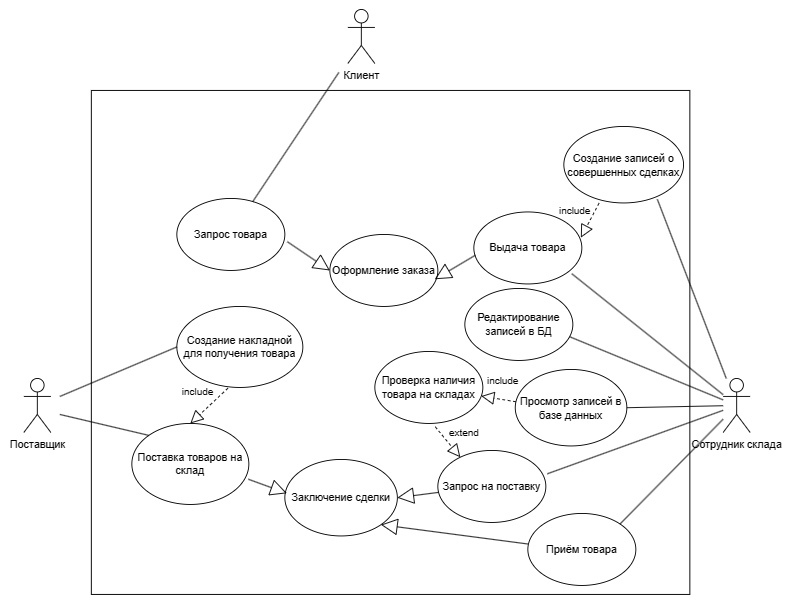
\includegraphics[width=1.0\linewidth]{UMLBD.jpg}

    Рисунок 1 - UML-Диаграмма
\end{center}



\begin{center}
\setlength{\tabcolsep}{3pt}
\resizebox{1.00\textwidth}{!}{
\newcolumntype{s}{>{\columncolor[HTML]{DDDDDD}} c}
  \begin{tabular}{ |s|c|c|c|c|c|c|c|c|c| } 
    \hline
    \rowcolor[HTML]{DDDDDD}
    & Категория & Клиент & Накладная & Отгрузка & Поставщик & Склад & Сотрудник & Товар & Товар на \\
    \rowcolor[HTML]{DDDDDD}
    & товаров && поставки &&&& склада && складе \\
    \hline
    Категория & \cellcolor[HTML]{AFAFAF} &&&&&&& Содержит & \\
    товаров & \cellcolor[HTML]{AFAFAF} &&&&&&&& \\ 
    \hline
    Клиент && \cellcolor[HTML]{AFAFAF} && Ожидает &&&&&\\ \hline
    Накладная &&& \cellcolor[HTML]{AFAFAF} && Выписывается & Предписывает & Подписывается & Описывает & \\
    поставки &&& \cellcolor[HTML]{AFAFAF} &&&&&& \\ 
    \hline
    Отгрузка && Ожидается && \cellcolor[HTML]{AFAFAF} && Отправляется & Контролируется & Состоит &\\ 
    \hline
    Поставщик &&& Выписывает && \cellcolor[HTML]{AFAFAF} &&& Поставляет & \\ 
    \hline
    Склад &&& Отвечает & Отправляет && \cellcolor[HTML]{AFAFAF} & Управляется && Хранит \\ 
    \hline
    Сотрудник &&& Подписывает & Контролирует && Управляет & \cellcolor[HTML]{AFAFAF} &&\\
    склада &&&&&&& \cellcolor[HTML]{AFAFAF} && \\ 
    \hline
    Товар & Содержится && Описывается & Входит & Поставляется &&& \cellcolor[HTML]{AFAFAF} & Дискретизирует \\ 
    \hline
    Товар на &&&&&& Хранится && Дискретизируется & \cellcolor[HTML]{AFAFAF} \\ 
    складе &&&&&&&&& \cellcolor[HTML]{AFAFAF} \\ 
    \hline
  \end{tabular}
}
\end{center}

\begin{center}
Рисунок 2 - Матрица связей
\end{center}

%\begin{justforlargetext}
%\large
%\textbf{Нормализация}\\
%\end{justforlargetext}

%\section{Нормализация (думаем)}
%\section{Денормализация (в процессе)}
%\textbf{Нормализация (думаем)}\\
%\textbf{Денормализация (в процессе)}\\


%\newpage
%\begin{justforlargetext}
%\large
%\textbf{Логическая модель}\\
%\end{justforlargetext}
\section{Нормализация}
\textbf{1НФ}
Составленная модель базы данных уже находится в первой нормальной форме, так как как в таблицах никогда не возникнет повторения строк, а в каждом столбце в одной ячейке находится единственное значение


\textbf{2НФ}
Также данная модель находится и во второй нормальной форме. Это обусловлено тем, что она находится в первой нормальной форме и выполняются условия второй нормальной формы. А именно все не ключевые значения зависят только от первичного ключа. (рисунок 3)


\textbf{3НФ}
Первоначально, разработанная модель не находится в третьей нормальной форме, поскольку есть транзитивная зависимость в таблице "сотрудник". Получалось так, что контактная информация о нем транзитивно зависела от имени, поэтому было принято решение вынести эти данные в отдельную сущность "Контакты". (рисунок 4)

\begin{center}
    \centering 
    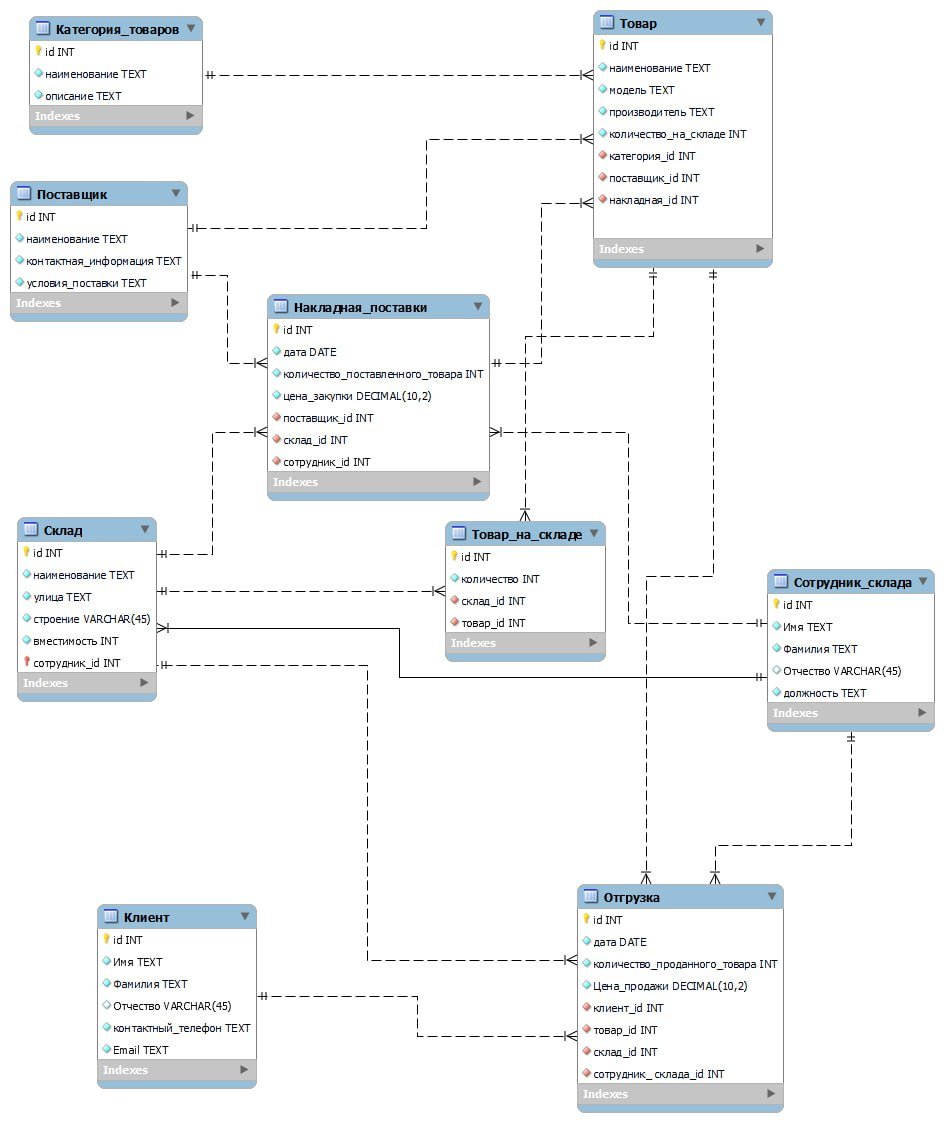
\includegraphics[width=1.0\linewidth]{second.jpg}
    \\Рисунок 3 - Схема БД в 2НФ.
\end{center}

\begin{center}
    \centering 
    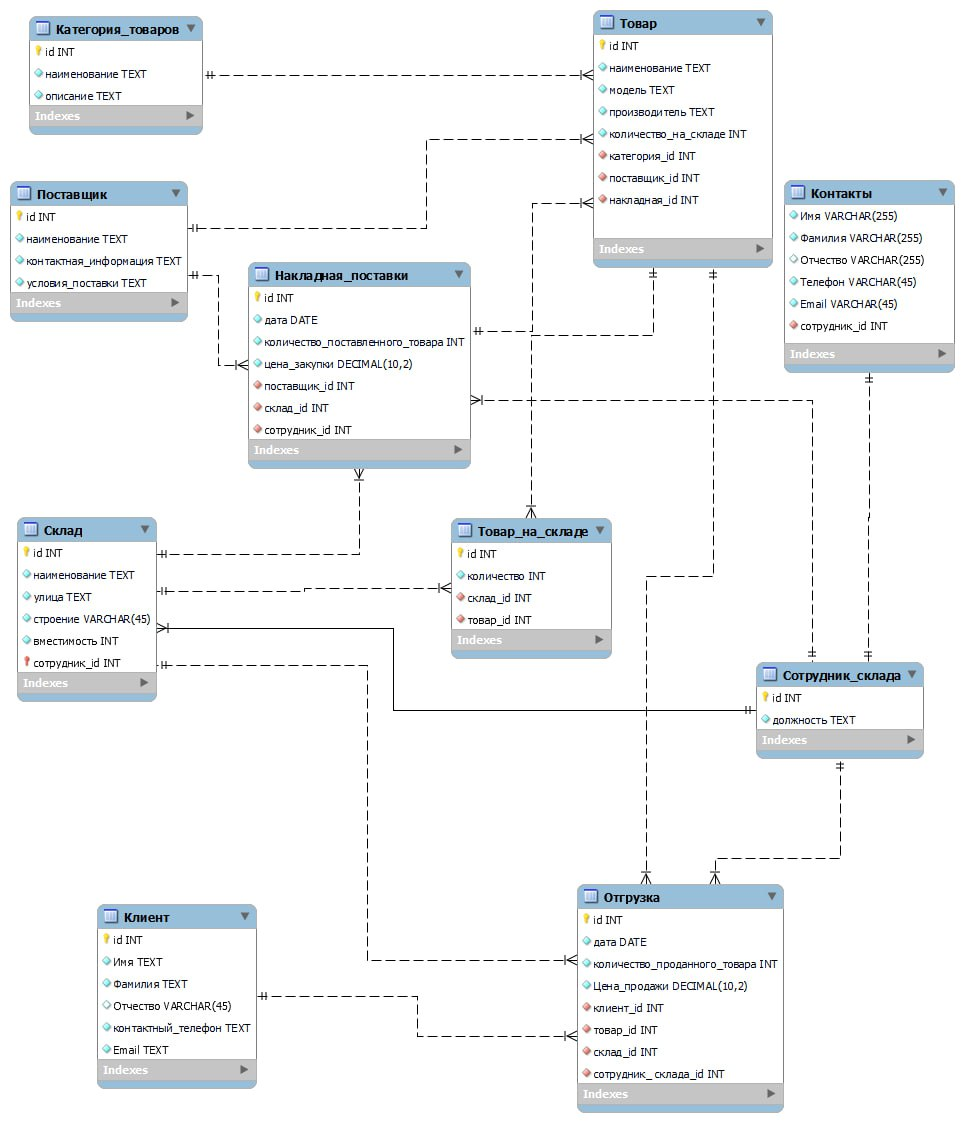
\includegraphics[width=1.0\linewidth]{third.jpg}
    \\Рисунок 4 - Схема БД в 3НФ.
\end{center}
\newpage
\section{Денормализация}

В контексте данной работы была реализована денормализация, посредством добавления трех различных атрибутов в сущности. А именно, атрибут "статистика склада" в сущнотсти "Склад", "количество принятого товара" в сущности "Сотрудник склада" и атрибут "всего покупок" в сущности "Клиент". (рисунок 5)


- атрибут 'количество принятого товара', показывающий, сколько товаров принял сотрудник


- атрибут 'всего покупок', показывающий, сколько товаров купил клиент


- атрибут 'статистика склада', показывающий, сколько в день на складе отгрузок и поставок


\begin{center}
    \centering 
    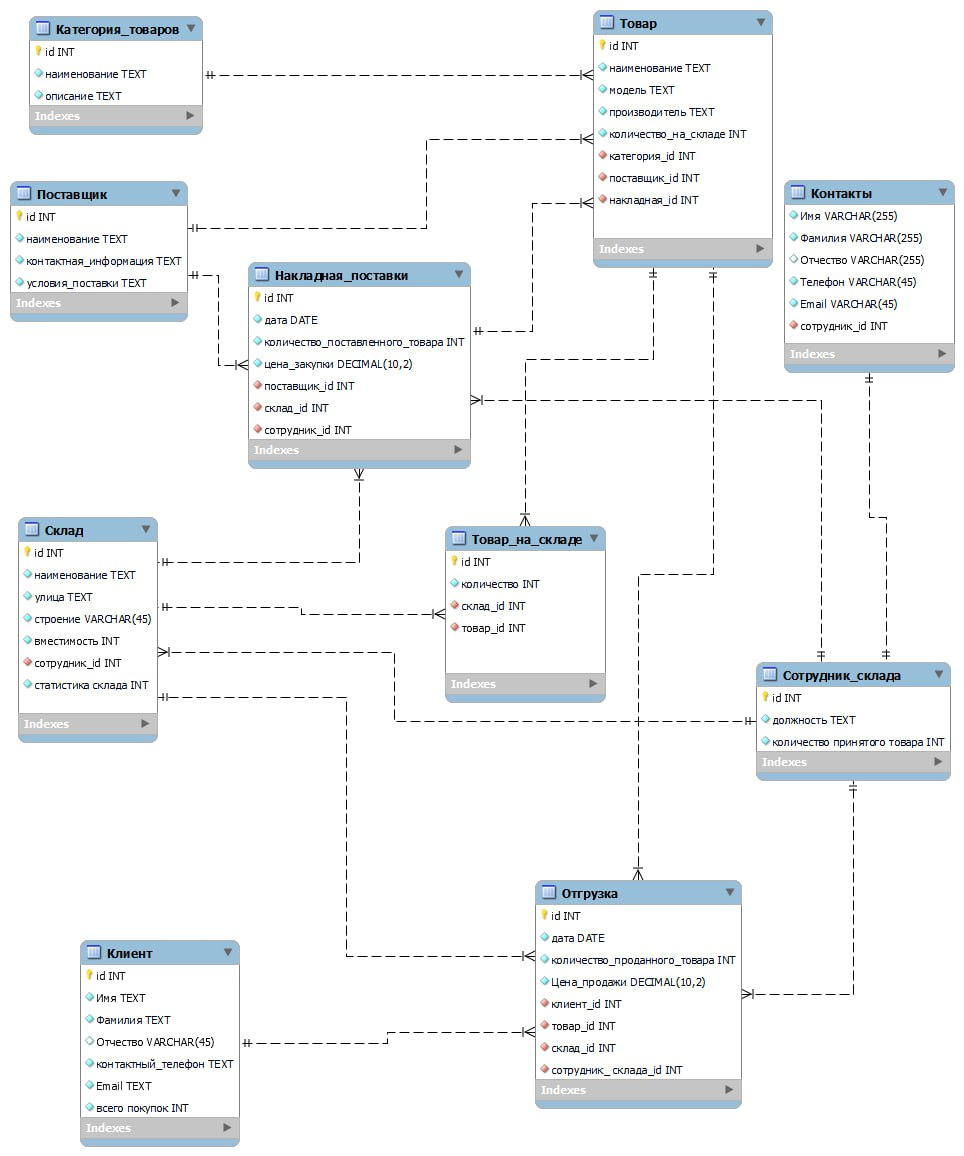
\includegraphics[width=1.0\linewidth]{denorm.jpg}
    \\Рисунок 5 - Денормализация.
\end{center}
\newpage
\section{йй}
В процессе разработки БД после нормализации до 3НФ сущности обновились. Были составлены новые таблицы для их описания: 

1. Товар


2. Клиент


3. Накладная поставки


4. Отгрузка


5. Поставщик


6. Склад


7. Сотрудник склада


8. Категория товаров 


9. Товар на складе


10. Контакты


\vspace{1em}
\noindent
Таблица 10 - Товар
\begin{center}
\begin{longtable}{ |m{3.3cm}|m{3cm}|m{6cm}|m{1.8cm}| } 
 \hline
 Атрибуты & Тип & Описание & Обяз. \\ [0.5ex] 
 \hline\hline
 id & INT & Первичный ключ & \# \\
 \hline
 Наименование & TEXT & Наименование товара & * \\
 \hline
 Модель & TEXT & Название модели & * \\
 \hline
 Производитель & TEXT & Производитель товара & *\\ 
 \hline
 Количество\_
 
 на\_складе & INT & Количество единиц товара на складе & * \\
 \hline
 Категория\_id & INT & Номер категории товара (внешний ключ) & * \\ 
 \hline
 Поставщик\_id & INT & Номер поставщика товара (внешний ключ) & * \\ 
 \hline
 Накладная\_id & INT & Номер накладной товара (внешний ключ) & * \\ 
 \hline

 \hline
\end{longtable}
\end{center}


\newpage

\noindent
Таблица 11 - Клиент
\begin{center}
\begin{longtable}{ |m{3.3cm}|m{3cm}|m{6cm}|m{1.8cm}| } 
 \hline
 Атрибуты & Тип & Описание & Обяз. \\ [0.5ex] 
 \hline\hline
 id & INT & Первичный ключ & \# \\
 \hline
 Имя & TEXT & Имя клиента & * \\
 \hline
 Фамилия & TEXT & Фамилия клиента & * \\
 \hline
 Отчество & TEXT & Отчество клиента & 0 \\
 \hline
 Контактный\_
 
 телефон & TEXT & Номер телефона клиента & [\#] \\
 \hline
 Email & TEXT & Электронная почта клиента & * \\
 \hline
\end{longtable}
\end{center}


\noindent
Таблица 12 - Накладная поставки
\begin{center}
\begin{longtable}{ |m{3.3cm}|m{3cm}|m{6cm}|m{1.8cm}| } 
 \hline
 Атрибуты & Тип & Описание & Обяз. \\ [0.5ex] 
 \hline\hline
 id & INT & Первичный ключ & \# \\
 \hline
 Дата & DATE & Дата поставки & * \\
 \hline
 Количество\_ 
 
 поставленного\_
 
 товара & INT & Количество единиц поставленного товара & * \\
 \hline
 Цена\_
 
 закупки & FLOAT & Цена закупки товаров  & * \\ 
 \hline
 Поставщик\_id & INT & Номер поставщика (внешний ключ) & * \\
 \hline
 Товар\_id & INT & Номер товара (внешний ключ) & * \\ 
 \hline
 Склад\_id & INT & Номер склада (внешний ключ) & * \\ 
 \hline
 Сотрудник\_id & INT & Номер сотрудника склада, подписавшего накладную (внешний ключ) & * \\ 
 \hline

 \hline
\end{longtable}
\end{center}


\newpage

\noindent
Таблица 13 - Отгрузка
\begin{center}
\begin{longtable}{ |m{3.3cm}|m{3cm}|m{6cm}|m{1.8cm}| } 
 \hline
 Атрибуты & Тип & Описание & Обяз. \\ [0.5ex] 
 \hline\hline
 id & INT & Первичный ключ & \# \\
 \hline
 Дата & DATE & Дата выполнения отгрузки & * \\
 \hline
 Количество\_
 
 проданного\_
 
 товара & INT & Количество проданных единиц товара & * \\
 \hline
 Цена\_
 
 продажи & FLOAT & Общая стоимость продажи товаров отгрузки & * \\
 \hline
 Клиент\_id & INT & Номер клиента (внешний ключ) & * \\
 \hline
 Товар\_id & INT & Номер отгружаемого товара (внешний ключ) & * \\
 \hline
 Склад\_id & INT & Номер склада (внешний ключ) & * \\
 \hline
 Сотрудник\_
 
 склада\_id & INT & Номер сотрудника склада, ответственного за отгрузку (внешний ключ) & * \\
 \hline
\end{longtable}
\end{center}



\noindent
Таблица 14 - Поставщик
\begin{center}
\begin{longtable}{ |m{3.3cm}|m{3cm}|m{6cm}|m{1.8cm}| } 
 \hline
 Атрибуты & Тип & Описание & Обяз. \\ [0.5ex] 
 \hline\hline
 id & INT & Первичный ключ & \# \\
 \hline
 Наименование & TEXT & Наименование компании поставщика & * \\
 \hline
 Контактная\_
 
 информация & TEXT & Контактная информация поставщика & * \\
 \hline
 Условия\_
 
 поставки & TEXT & Условия поставки товаров от поставщика & * \\
 \hline
\end{longtable}
\end{center}


\newpage
\noindent
Таблица 15 - Склад
\begin{center}
\begin{longtable}{ |m{3.3cm}|m{3cm}|m{6cm}|m{1.8cm}| } 
 \hline
 Атрибуты & Тип & Описание & Обяз. \\ [0.5ex] 
 \hline\hline
 id & INT & Первичный ключ & \# \\
 \hline
 Наименование & TEXT & Название склада & * \\
 \hline
 Улица & TEXT & Название улицы, на которой находится склад & * \\
 \hline
 Строение & TEXT & Строение, в котором находится склад & * \\
 \hline
 Вместимость & INT & Вместимость склада & * \\
 \hline
\end{longtable}
\end{center}



\noindent
Таблица 16 - Сотрудник склада
\begin{center}
\begin{longtable}{ |m{3.3cm}|m{3cm}|m{6cm}|m{1.8cm}| } 
 \hline
 Атрибуты & Тип & Описание & Обяз. \\ [0.5ex] 
 \hline\hline
 id & INT & Первичный ключ & \# \\
 \hline
 Должность & TEXT & Должность сотрудника & * \\
 \hline
\end{longtable}
\end{center}



\noindent
Таблица 17 - Категория товаров
\begin{center}
\begin{longtable}{ |m{3.3cm}|m{3cm}|m{6cm}|m{1.8cm}| } 
 \hline
 Атрибуты & Тип & Описание & Обяз. \\ [0.5ex] 
 \hline\hline
 id & INT & Первичный ключ & \# \\
 \hline
 Наименование & TEXT & Наименование категории & * \\
 \hline
 Описание & TEXT & Описание категории & * \\
 \hline
\end{longtable}
\end{center}


\newpage

\noindent
Таблица 18 - Товар на складе
\begin{center}
\begin{longtable}{ |m{3.3cm}|m{3cm}|m{6cm}|m{1.8cm}| } 
 \hline
 Атрибуты & Тип & Описание & Обяз. \\ [0.5ex] 
 \hline\hline
 id & INT & Первичный ключ & \# \\
 \hline
 Количество & INT & Количество товара на складе & * \\
 \hline
 Склад\_id & INT & Номер склада (внешний ключ) & * \\
 \hline
 Товар\_id & INT & Номер товара (внешний ключ) & * \\
 \hline
\end{longtable}
\end{center}


\noindent
Таблица 19 - Контакты
\begin{center}
\begin{longtable}{ |m{3.3cm}|m{3cm}|m{6cm}|m{1.8cm}| } 
 \hline
 Атрибуты & Тип & Описание & Обяз. \\ [0.5ex] 
 \hline\hline
 Имя & TEXT & Имя сотрудника & \# \\
 \hline
 Фамилия & TEXT & Фамилия сотрудника & \# \\
 \hline
 Отчество & TEXT & Отчество сотрудника & \# \\
 \hline
 Телефон & TEXT & Телефон сотрудника & [\#] \\
 \hline
 Email & TEXT & Электронная почта сотрудника & [\#] \\
 \hline
 Сотрудник\_id & INT & Идентификационный номер сотрудника(внешний ключ) & [\#] \\
 \hline
\end{longtable}
\end{center}


\newpage

\section{Создание документа сопоставления моделей}
На основании ERD-диаграммы было разработана методика сопоставления таблиц, представляющая преобразование терминологии логической модели данных в термины физической. Сопоставление логической и физической моделей данных выведено в таблицах 20-29.


\noindent
Таблица 20 - Products categories PCS
\begin{center}
\begin{longtable}{ |m{1.3cm}|m{2.7cm}|m{4.5cm}|m{3.5cm}|m{1.8cm}| } 
 \hline
 Key type & Optionality & Column name & Data type & Size \\ [0.5ex] 
 \hline\hline
 pk & \# & id & INT & 8 \\
 \hline
  & * & Наименование & VARCHAR(45) & 46 \\
 \hline
  & * & Описание & VARCHAR(45) & 46 \\
 \hline
\end{longtable}
\end{center}


\noindent
Таблица 21 - Provider PVR
\begin{center}
\begin{longtable}{ |m{1.3cm}|m{2.7cm}|m{4.5cm}|m{3.5cm}|m{1.8cm}| } 
 \hline
 Key type & Optionality & Column name & Data type & Size \\ [0.5ex] 
 \hline\hline
 pk & \# & id & INT & 8 \\
 \hline
  & * & Наименование & VARCHAR(45) & 46 \\
 \hline
  & * & Контактная\_
  
  информация & VARCHAR(45) & 46 \\
  \hline
  & * & Условия\_поставки & VARCHAR(45) & 46 \\
 \hline
\end{longtable}
\end{center}


\newpage

\noindent
Таблица 22 - Products PDS
\begin{center}
\begin{longtable}{ |m{1.3cm}|m{2.7cm}|m{4.5cm}|m{3.5cm}|m{1.8cm}| } 
 \hline
 Key type & Optionality & Column name & Data type & Size \\ [0.5ex] 
 \hline\hline
 pk & \# & id & INT & 8 \\
 \hline
  & * & Наименование & VARCHAR(45) & 46 \\
 \hline
  & * & Модель & VARCHAR(45) & 46 \\
 \hline
  & * & Производитель & VARCHAR(45) & 46 \\
 \hline
  & * & Количество\_
 
 на\_складе & INT & 8 \\
 \hline
 fk & * & Категория\_id & INT & 8 \\
 \hline
 fk & * & Поставщик\_id & INT & 8 \\
 \hline
 fk & * & Накладная\_id & INT & 8 \\
 \hline
\end{longtable}
\end{center}


\noindent
Таблица 23 - Delivery invoice DIV
\begin{center}
\begin{longtable}{ |m{1.3cm}|m{2.7cm}|m{4.5cm}|m{3.5cm}|m{1.8cm}| } 
 \hline
 Key type & Optionality & Column name & Data type & Size \\ [0.5ex] 
 \hline\hline
 pk & \# & id & INT & 8 \\
 \hline
  & * & Дата & DATE & 8 \\
 \hline
  & * & Количество\_
  
 поставленного\_
  
 товара & INT & 8 \\
 \hline
  & * & Цена\_
  
 закупки & DECIMAL(10,2) & 12 \\
 \hline
 fk & * & Поставщик\_id & INT & 8 \\
 \hline
 fk & * & Склад\_id & INT & 8 \\
 \hline
 fk & * & Сотрудник\_id & INT & 8 \\
 \hline
\end{longtable}
\end{center}


\newpage

\noindent
Таблица 24 - Warehouse WHS
\begin{center}
\begin{longtable}{ |m{1.3cm}|m{2.7cm}|m{4.5cm}|m{3.5cm}|m{1.8cm}| } 
 \hline
 Key type & Optionality & Column name & Data type & Size \\ [0.5ex] 
 \hline\hline
 pk & \# & id & INT & 8 \\
 \hline
  & * & Наименование & VARCHAR(45) & 46 \\
 \hline
  & * & Улица & VARCHAR(45) & 46 \\
 \hline
  & * & Строение & VARCHAR(45) & 46 \\
 \hline
  & * & Вместимость & INT & 8 \\
 \hline
 fk & * & Сотрудник\_id & INT & 8 \\
 \hline
\end{longtable}
\end{center}


\noindent
Таблица 25 - Products on stock - POS
\begin{center}
\begin{longtable}{ |m{1.3cm}|m{2.7cm}|m{4.5cm}|m{3.5cm}|m{1.8cm}| } 
 \hline
 Key type & Optionality & Column name & Data type & Size \\ [0.5ex] 
 \hline\hline
 pk & \# & id & INT & 8 \\
 \hline
  & * & Количество & INT & 8 \\
 \hline
 fk & * & Склад\_id & INT & 8 \\
 \hline
 fk & * & Товар\_id & INT & 8 \\
 \hline
\end{longtable}
\end{center}


\noindent
Таблица 26 - Warehouse employee WEE
\begin{center}
\begin{longtable}{ |m{1.3cm}|m{2.7cm}|m{4.5cm}|m{3.5cm}|m{1.8cm}| } 
 \hline
 Key type & Optionality & Column name & Data type & Size \\ [0.5ex] 
 \hline\hline
 pk & \# & id & INT & 8 \\
 \hline
  & * & Должность & VARCHAR(45) & 46 \\
 \hline
\end{longtable}
\end{center}


\newpage

\noindent
Таблица 27 - Client CLT
\begin{center}
\begin{longtable}{ |m{1.3cm}|m{2.7cm}|m{4.5cm}|m{3.5cm}|m{1.8cm}| } 
 \hline
 Key type & Optionality & Column name & Data type & Size \\ [0.5ex] 
 \hline\hline
 pk & \# & id & INT & 8 \\
 \hline
  & \# & Имя & VARCHAR(45) & 46 \\
 \hline
  & * & Фамилия & VARCHAR(45) & 46 \\
 \hline
  & 0 & Отчество & VARCHAR(45) & 46 \\
 \hline
 uk & [\#] & Контактный\_
 
 телефон & VARCHAR(45) & 46 \\
 \hline
  & * & Email & VARCHAR(45) & 46 \\
 \hline
\end{longtable}
\end{center}


\noindent
Таблица 28 - Shipment SPT
\begin{center}
\begin{longtable}{ |m{1.3cm}|m{2.7cm}|m{4.5cm}|m{3.5cm}|m{1.8cm}| } 
 \hline
 Key type & Optionality & Column name & Data type & Size \\ [0.5ex] 
 \hline\hline
 pk & \# & id & INT & 8 \\
 \hline
  & * & Дата & DATE & 8 \\
 \hline
  & * & Количество\_
  
  проданного\_
  
  товара & INT & 8 \\
 \hline
  & * & Цена\_
  
  продажи & DECIMAL(10,2) & 12 \\
% \hline
%\end{longtable}
%\hfill Продолжение таблицы 31
%\begin{longtable}{ |m{1.3cm}|m{2.7cm}|m{4.5cm}|m{3.5cm}|m{1.8cm}| }
 \hline
 fk & * & Клиент\_id & INT & 8 \\
 \hline
 fk & * & Товар\_id & INT & 8 \\
 \hline
 fk & * & Склад\_id & INT & 8 \\
 \hline
 fk & * & Сотрудник\_
 
 склада\_id & INT & 8 \\
 \hline
\end{longtable}
\end{center}


\newpage

\noindent
Таблица 29 - Contacts CTS
\begin{center}
\begin{longtable}{ |m{1.3cm}|m{2.7cm}|m{4.5cm}|m{3.5cm}|m{1.8cm}| } 
 \hline
 Key type & Optionality & Column name & Data type & Size \\ [0.5ex] 
 \hline\hline
 pk & \# & Имя & VARCHAR(255) & 256 \\
 \hline
 pk & \# & Фамилия & VARCHAR(255) & 256 \\
 \hline
  & 0 & Отчество & VARCHAR(255) & 256 \\
 \hline
 uk & \# & Телефон & VARCHAR(45) & 46 \\
 \hline
  & \# & Email & VARCHAR(45) & 46 \\
 \hline
 fk & [\#] & Сотрудник\_id & VARCHAR(45) & 46 \\
 \hline
\end{longtable}
\end{center}


\conclusions
%\chapter{ЗАКЛЮЧЕНИЕ}


В рамках нашего проекта мы сфокусировались на разработке базы данных для управления магазином бытовой техники. Этот процесс включал несколько ключевых этапов:

1. Проведён глубокий анализ требований и особенностей, связанных с управлением магазином бытовой техники. Рассмотрены основные процессы бизнеса, определили роли участников системы и выделили основные объекты, с которыми мы будем работать.

2. На основе полученных данных и диаграммы бизнес-процессов мы выявили ключевые объекты и их взаимосвязи в базе данных. Эти объекты представляют собой, например, товары, поставщиков, заказы, клиентов и другие.

3. Определены основные атрибуты и идентификаторы для каждой сущности. Строили ER- и UML-диаграммы для наглядного представления логической структуры данных и создали дополнительные таблицы для обработки сложных связей.

4. Приведены данные к более структурированному виду с помощью процесса нормализации, устранив избыточность и предотвратив связи между атрибутами.

5. Для оптимизации работы базы данных мы внесли дополнительные данные в некоторые таблицы, чтобы обеспечить более быстрый доступ к информации.

6. На основе логической модели была создана физическая структура базы данных. Мы разработали различные SQL-запросы и применили их для проверки работоспособности базы данных, используя язык запросов SQL.

Таким образом, наша работа привела к созданию готовой базы данных MySQL, которая будет эффективно управлять информацией о товарах и операциях в магазине бытовой техники.


\begin{thebibliography}

\bibitem{bib1} Wikipedia: официальный сайт: 
\url{https://ru.wikipedia.org/wiki/База_данных} (Дата обращение 31.05.2023)

\bibitem{bib2} Wikipedia: официальный сайт: \url{https://ru.wikipedia.org/wiki/SQL} (Дата обращение 31.05.2023)

\bibitem{bib3} MySQL Workbench: официальный сайт: \url{https://dev.mysql.com/downloads/workbench/} (Дата обращение 10.12.2023)

\bibitem{bib3} Ссылка на Google Drive c логической моделью и итоговым SQL скриптом: \url{https://kurl.ru/gHmvD} (Дата обращение 10.12.2023)

\end{thebibliography}

\chapter{Приложение: Физическая модель данных}
%Была реализована физическая модель данных.
Для создания физической модели базы данных, спроектированная
логическая модель была перенесена в SQL-скрипт с помощью средств средств
среды разработки MySQL Workbench. Далее производилось подключение MySQL Workbench к СУБД в разделе «Database → Manage Connections».
Адресом сервера в данном случае был (127.0.0.1)(локальный компьютер). Port стандартный: 3306
Также была произведена синхронизация структуры базы данных на сервере и спроектированной ранее логической модели.


\begin{center}
    \centering
    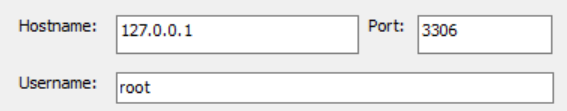
\includegraphics[width=0.8\linewidth]{host.png}
    \\Рисунок 6 - Адрес SQL сервера с БД
\end{center} 


\begin{center}
    \centering
    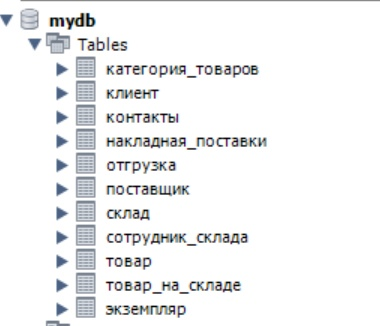
\includegraphics[width=0.5\linewidth]{image5.png}
    \\Рисунок 7 - Подключение MySQL Workbench к СУБД.
\end{center}

\section{SQL - запросы}
В данном разделе были разработаны запросы к созданной базе данных в
целях закрепления на практике знаний о языке SQL. С точки зрения реализации, язык SQL представляет собой набор операторов, которые делятся на определенные группы и у каждой группы есть свое назначение. В сокращенном виде эти группы называются DQL, DML, каждая из групп характеризуется определенными операторами. На рисунках ниже представлены несколько запросов использования некоторых операторов с пояснениями (рисунки 8-11).


Первая группа запросов позволяет удалять/просматривать/добавлять инфорацию в таблицу ''Товар''. В этих запросах используется команда ''SELECT'' из DQL и ''INSERT'' с ''DELETE'' из DML (рисунок 8). 
\begin{center}
    \centering
    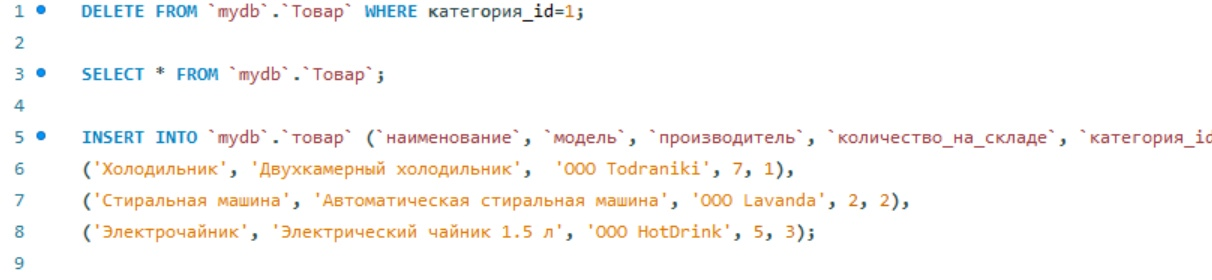
\includegraphics[width=1.0\linewidth]{image1.png}
    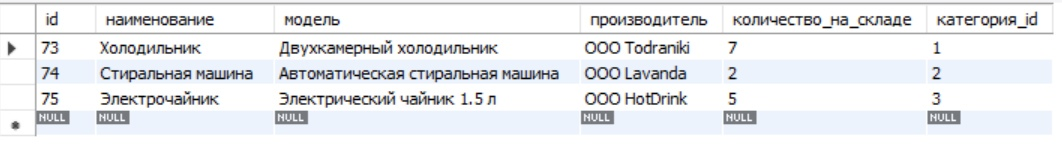
\includegraphics[width=1.0\linewidth]{image.png}
    %\caption{Рисунок 4 - ...}
    %\small
    \\Рисунок 8 - Общие команды для работы с таблицами (1)
    %\label{fig:enter-label}
\end{center}

Второй запрос позволяет выводить определенные значения  из таблицы ''Сотрудник склада'', а именно графу "должность". В данном запросе используются операторы ''SELECT'' и ''FROM''. Запрос, позволяющий просмотреть должность сотрудников, которые работают в компании (рисунок 9).
\begin{center}
    \centering 
    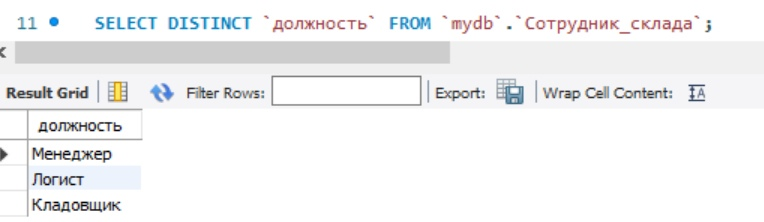
\includegraphics[width=1.0\linewidth]{image2.png}
    \\Рисунок 9 - Общие команды для работы с таблицами (2)
\end{center}


Данный запрос позволяет объединить информацию из нескольких таблиц, сделав её сводной, посредством оператора ''JOIN''. Данный запрос объединяет определенные графы из таблиц ''Отгрузка'' и ''Клиент''. По итогу запрос выводит информацию о клиенте и дате отгрузки товара для этого клиента (рисунок 10).
\begin{center}
    \centering
    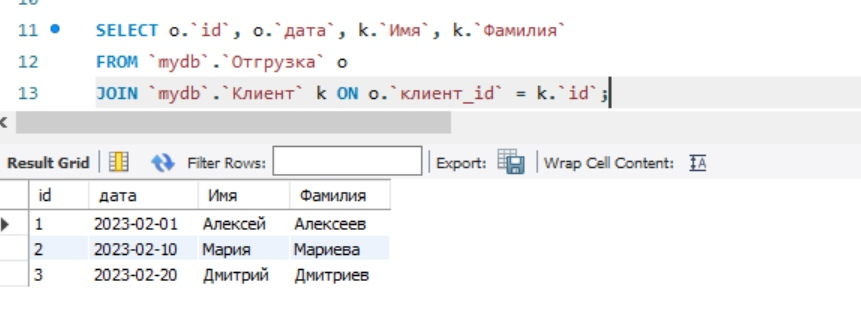
\includegraphics[width=1.0\linewidth]{image3.png}
    \\Рисунок 10 - Запрос (1) c оператором "JOIN" 
\end{center}


Еще один запрос с оператором ''JOIN'', который выводит количество поставленного товара, которое было принято определенном сотрудником склада и дата подписания накладной поставки (рисунок 11). Данный запрос объединяет определенные графы из таблиц ''Сотрудник склада'' и ''Накладная поставки''. 
\begin{center}
    \centering
    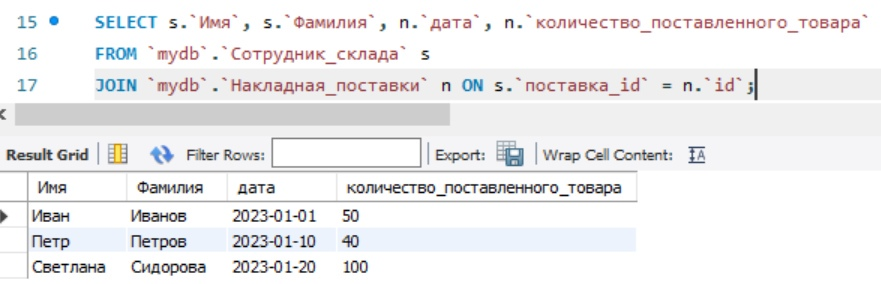
\includegraphics[width=1.0\linewidth]{image4.png}
    \\Рисунок 11 - Запрос (2) c оператором "JOIN"
\end{center}




\end{document}
